\documentclass[letterpaper,12pt,openright,oneside]{article}
% \documentclass[book,12pt,openright,oneside]{article}
%%%%%%%%%%%%%%%%%%%%%%%%%%%%%%%%%%%%%%%%%%%
\renewcommand{\familydefault}{\sfdefault} % Arial font
\setlength{\parindent}{16mm} % sangria de 1.6 cm
%%%%%%%%%%%%%%%%%%%%%%%%%%%%%%%%%%%%%%%%%%%
% \usepackage[left=3cm,top=3cm,right=2cm,nohead,foot=.5cm]{geometry}
% \usepackage[left=3cm,top=3cm,right=3cm,nohead,foot=2.5cm]{geometry}
\usepackage[left=2cm,top=2cm,right=2cm,nohead,foot=3cm]{geometry}
\usepackage[spanish,mexico]{babel}
%\usepackage[spanish]{babel}
%\usepackage[latin1]{inputenc}
%%%%%%%%%%%%%%%%%%%%%%%%%%%%%%%%%%%%%%%%%%%%%%%%%%%%%%%%
\usepackage{listings} % Using listings to highlight code
\usepackage{xcolor}

\definecolor{codegreen}{rgb}{0,0.6,0}
\definecolor{codegray}{rgb}{0.5,0.5,0.5}
\definecolor{codepurple}{rgb}{0.58,0,0.82}
\definecolor{backcolour}{rgb}{0.95,0.95,0.92}

\lstdefinestyle{mystyle}{
    backgroundcolor=\color{backcolour},   
    commentstyle=\color{codegreen},
    keywordstyle=\color{magenta},
    numberstyle=\tiny\color{codegray},
    stringstyle=\color{codepurple},
    basicstyle=\ttfamily\footnotesize,
    breakatwhitespace=false,         
    breaklines=true,                 
    captionpos=b,                    
    keepspaces=true,                 
    numbers=right,                    
    numbersep=5pt,                  
    showspaces=false,                
    showstringspaces=false,
    showtabs=false,                  
    tabsize=2
}

\lstset{style=mystyle}
%%%%%%%%%%%%%%%%%%%%%%%%%%%%%%%%%%%%%%%%%%%%%%%%%%%%%%%%
\usepackage{chngpage}
\usepackage{lineno} %paquete para agregar números a cada linea
\usepackage{times}
\usepackage{url}
\usepackage{pdflscape}
\usepackage[utf8]{inputenc}
\usepackage{graphicx}
\graphicspath{ {images/} }
\usepackage{color}
\usepackage{babelbib}
% \usepackage{subfig}
\usepackage{subcaption} %paquete para tener multiple imagenes
\usepackage{amsmath,amssymb,amsthm} 
% assumes amsmath package installed
%\usepackage[document]{ragged2e}
\usepackage{hyperref}
\hypersetup{
colorlinks=true,
citecolor=black,
urlcolor=blue,
}
\urlstyle{rm}
\expandafter\def\expandafter\UrlBreaks\expandafter{\UrlBreaks%  save the current one
  \do\a\do\b\do\c\do\d\do\e\do\f\do\g\do\h\do\i\do\j%
  \do\k\do\l\do\m\do\n\do\o\do\p\do\q\do\r\do\s\do\t%
  \do\u\do\v\do\w\do\x\do\y\do\z\do\A\do\B\do\C\do\D%
  \do\E\do\F\do\G\do\H\do\I\do\J\do\K\do\L\do\M\do\N%
  \do\O\do\P\do\Q\do\R\do\S\do\T\do\U\do\V\do\W\do\X%
  \do\Y\do\Z}
\newcommand{\grad}{$^{\circ}$}
\usepackage{multirow}
\usepackage{todonotes}
\usepackage{makecell}
\usepackage{enumitem}
\usepackage{array}
\usepackage{amsmath}
\usepackage{tabularx}
\usepackage{pdfpages} % \includepdf[pages=-]{myfile.pdf}
\usepackage{bm,upgreek}
\usepackage{afterpage}
\usepackage{gensymb} % Generic symbols for both text and math mode
\usepackage{float}
\usepackage{marvosym}
\usepackage{ragged2e}
\definecolor{light-gray}{gray}{.7}
%\spanishdecimal{.}

%-------------------------------------------
\theoremstyle{plain}
\newtheorem{theorem}{Theorem}
\newcommand{\parcial}[2]{\frac{\partial{#1}}{\partial{#2}}}
\newtheorem{lemma}{Lema}[subsection]
%\newtheorem{proof}[theorem]{Proof}
%\theoremstyle{definition}
\newtheorem{defn}{Definition}
\newtheorem{remark}{Remark}
%\newcommand{\parcial}[2]{\frac{\partial{#1}}{\partial{#2}}}
\DeclareMathOperator{\sign}{sign}
\newcommand{\m}[1]{\mathbf{#1}}
\DeclareMathOperator{\diag}{diag}

\renewcommand{\baselinestretch}{1.5} % interlineado

\newcolumntype{P}[1]{>{\centering\arraybackslash}p{#1}}
\setlength {\marginparwidth }{2cm} 
%%%%%%%%%%%%%%%%%%%%%%%%%%%%%%%%%%%%%
\renewcommand\thesection{\Roman{section}} %  letters for sections
% \renewcommand*{\thesubsection}{\null{}}
\renewcommand*{\thesubsection}{\alph{subsection}}
\renewcommand*{\thesubsubsection}{\null{}}
%%%%%%%%%%%%%%%%%%%%%%%%%%%%%%%%%%%%%
%%%%%%%%%%%%%%%%%%%%%%%%%%%%%%%%%%%%%
\begin{document}

\begin{titlepage}
\begin{center}

% Upper part of the page. The '~' is needed because \\
% only works if a paragraph has started.

\textsc{\LARGE Tecnológico Nacional de México}\\[0.6 cm]

\includegraphics[width=0.15\textwidth]{img/ITQNN.jpg}~\\[0.45cm]
\textsc{\Large Instituto Tecnológico de Querétaro \\ \large{Ingeniería Industrial}}\\[0.5 cm]
\textsc{\large Proyecto integrador \\ (Febrero 2024 - Mayo 2024)}\\[4.5cm]

{ 
\huge \bfseries
%%%%%%%%%%%%%%%%%%%%%%%%%%%%%%%%%%%%%%%%
Estudio del Trabajo II
%%%%%%%%%%%%%%%%%%%%%%%%%%%%%%%%%%%%%%%%
\\[0.4cm] }
\vspace*{1.5cm}

% Author and supervisor
\textbf{Profesor:} Dr. Luis Alberto Ángeles Hurtado\\\vspace*{0.5cm}

\raggedright
% $^{1}$ Instituto Tecnológico de Querétaro.\\

\vfill
\centering
% Bottom of the page
% {\large \today}
%{\large 5 de diciembre de 2020}
\end{center}
\end{titlepage}

% \newpage
%%%%
\hypersetup{linkcolor=black}
% \newpage
% 
\renewcommand\contentsname{\centering \'INDICE}
\tableofcontents
\newpage
\linenumbers
% 
%
\section{Introducción}
El estudio del trabajo y el análisis de operaciones son disciplinas fundamentales en el ámbito de la ingeniería industrial y la gestión de operaciones. Estas áreas se centran en comprender, mejorar y optimizar los procesos de trabajo en una variedad de entornos, desde la manufactura hasta los servicios.

El estudio del trabajo se enfoca en analizar y mejorar la forma en que se realizan las tareas individuales dentro de un proceso. Esto implica examinar cada paso de una actividad laboral, desde cómo se lleva a cabo hasta cuánto tiempo lleva, con el objetivo de aumentar la eficiencia, reducir los costos y mejorar las condiciones laborales.

El análisis de operaciones, por otro lado, se centra en el estudio de procesos completos o sistemas de trabajo. Esto incluye la identificación y evaluación de los diferentes elementos que componen un proceso, como el flujo de trabajo, la distribución de instalaciones, el manejo de materiales y la utilización de recursos humanos y tecnológicos. El objetivo del análisis de operaciones es mejorar la productividad, la calidad y la rentabilidad de una organización mediante la optimización de sus operaciones.

Ambas disciplinas son vitales para las organizaciones que buscan mantenerse competitivas en un entorno empresarial en constante cambio. Al aplicar técnicas de estudio del trabajo y análisis de operaciones, las empresas pueden identificar áreas de mejora, eliminar desperdicios, reducir los tiempos de ciclo, mejorar la calidad del producto o servicio y aumentar la satisfacción del cliente.

En esta introducción, exploraremos los principios básicos del estudio del trabajo y el análisis de operaciones, así como sus aplicaciones en diferentes industrias y sectores. Además, examinaremos las herramientas y técnicas utilizadas en estas disciplinas, y cómo pueden contribuir al éxito y la eficiencia de una organización.
\section {Desarrollo}

subtema: 
\section{Definiciones}

El estudio del trabajo, también conocido como ingeniería de métodos o ingeniería de tiempos y movimientos, es una disciplina que se enfoca en analizar, mejorar y optimizar los procesos de trabajo en una organización. Su objetivo principal es aumentar la eficiencia y la productividad, reducir los costos y mejorar las condiciones laborales.

En el estudio del trabajo se utilizan diversas técnicas y herramientas, como el análisis de tiempos y movimientos, el diseño de estaciones de trabajo ergonómicas, el balanceo de líneas de producción, el diseño de sistemas de incentivos y recompensas, entre otros.

Este campo de estudio es fundamental en áreas como la manufactura, la logística, los servicios y cualquier otra actividad que implique la realización de tareas repetitivas o procesos de producción. Además, el estudio del trabajo contribuye a mejorar la calidad de vida de los trabajadores al reducir la fatiga y el estrés laboral, así como a aumentar la competitividad de las empresas en el mercado.
Los Therbligs
Los therbligs son una serie de símbolos inventados por Frank Bunker Gilbreth, Sr. y Lillian Moller Gilbreth en la década de 1920. Estos símbolos se utilizan para representar movimientos básicos en el trabajo, tanto físicos como mentales. Los Gilbreth eran pioneros en el estudio de la eficiencia en el trabajo y en el desarrollo de métodos para mejorar la productividad y reducir la fatiga en los trabajadores.


Los therbligs se utilizan en la industria y la ingeniería para analizar y mejorar los procesos de trabajo. Cada therblig representa una acción específica, como agarrar, mover, inspeccionar, buscar, etc. Al estudiar y analizar los therbligs involucrados en un proceso de trabajo, los ingenieros y gerentes pueden identificar áreas de ineficiencia y encontrar formas de optimizar el proceso, reducir los tiempos de ciclo y mejorar la productividad.

Los therbligs son una herramienta útil para el diseño de estaciones de trabajo, la planificación de procesos de fabricación y la capacitación de empleados. Ayudan a descomponer las tareas complejas en sus elementos más básicos, lo que facilita la identificación de áreas de mejora y la implementación de cambios para aumentar la eficiencia y la calidad del trabajo.
Los Therbligs se dividen en dos ramas: los efectivos y los inefectivos. Los efectivos agregan un valor a cualquier operación, mientras que los inefectivos sólo agregan costos.

Los Therbligs se dividen en dos ramas: los efectivos y los inefectivos. Los efectivos agregan un valor a cualquier operación, mientras que los inefectivos sólo agregan costos.

La importancia de su estudio se ve primordialmente reflejada en los procesos industriales que requieran de alto número de repetición. En el diseño del trabajo lo más importante es que cada acción que lleve a cabo la empresa o industria brinde algún valor agregado al proceso. Por tanto el objetivo de cualquier industria es eliminar cualquier Therblig inefectivo que se encuentre en uso y, de esta forma, mejorar su productividad.

Después de dividir la operación en el número de Therbligs necesarios es importante determinar los tipos de Therbligs con los que se hayan estado trabajando, los efectivos y los inefectivos. Una vez determinados los Therbligs lo usual sería realizar un mapa de operaciones que indique el flujo de procesos que existe en la industria. Posteriormente se analiza la información, se busca la pronta y posible eliminación de los Therbligs inefectivos y, de ser necesario, se busca una forma de rediseñar el proceso, recordando que el máximo objetivo de este estudio es el encontrar las condiciones más adecuadas para lograr maximizar la productividad.

Los movimientos básicos elementales
Un movimiento elemental básico es el conjunto de los movimientos requeridos para que un trabajador complete una tarea manual, operación o tarea.
Los Therbligs eficientes son:
1. Alcanzar. (Corresponde al movimiento de una mano vacía, sin barreras, hacia un objeto o retirándola de él)
2. Tomar. (Movimiento que hace la mano al cerrar los dedos rodeando una pieza y vincularla a una operación)
3. Mover. (Comienza cuando la mano con carga se mueve hacia un sitio y termina cuando llega a su destino)
4. Soltar. (Ocurre cuando el operario abandona el control del objeto. Se ejecuta en el más breve tiempo )
5. Ensamblar. (Es la división que ocurre cuando se reúnen dos o más piezas de ensamble)
6. Desmontar. (Ocurre cuando se separan piezas de ensamble unidas entre sí)
7. Usar. (Es en absoluto objetivo, ocurre cuando una o las dos manos intervienen una pieza durante el ciclo)
8. Preparar posición. (Es colocar un objeto en un sitio fijo para que esté disponible cuando se necesite )
Los Therbligs ineficientes son:
1. Planear. (Es el estado mental que se presenta cuando la persona se detiene para fijar la acción a seguir)
2. Buscar. (Se debe eliminar. Las estaciones de trabajo bien planeadas permiten que el trabajo no se interrumpa)
3. Seleccionar. (Se debe eliminar del ciclo mediante una mejor distribución en la estación de trabajo)
4. Inspeccionar. (Se incluye para asegurar una calidad aceptable, es una verificación realizada por el trabajador)
5. Demora evitable. (Todo tiempo muerto que ocurre durante el ciclo y que sólo depende del operario)
6. Demora inevitable. (Interrupción que el operario no puede evitar)
7. Colocar en posición. (Radica en situar un objeto de modo que quede dispuesto en su sitio específico)
8. Descansar. (Aparece rara vez en un ciclo de trabajo, surge de la necesidad del operario para reponer la fatiga)
9. Sostener. (Ocurre cuando una mano soporta algo, mientras la otra ejecuta tarea, se impide con buen diseño)


La importancia de su estudio se ve primordialmente reflejada en los procesos industriales que requieran de alto número de repetición. En el diseño del trabajo lo más importante es que cada acción que lleve a cabo la empresa o industria brinde algún valor agregado al proceso. Por tanto el objetivo de cualquier industria es eliminar cualquier Therblig inefectivo que se encuentre en uso y, de esta forma, mejorar su productividad.

Después de dividir la operación en el número de Therbligs necesarios es importante determinar los tipos de Therbligs con los que se hayan estado trabajando, los efectivos y los inefectivos. Una vez determinados los Therbligs lo usual sería realizar un mapa de operaciones que indique el flujo de procesos que existe en la industria. Posteriormente se analiza la información, se busca la pronta y posible eliminación de los Therbligs inefectivos y, de ser necesario, se busca una forma de rediseñar el proceso, recordando que el máximo objetivo de este estudio es el encontrar las condiciones más adecuadas para lograr maximizar la productividad.


% \begin{figure}[H]
%     \centering
%     \includegraphics[trim = {6mm 150mm 20mm 14mm},clip,scale=0.68]{img/fig_1.pdf}
%     \caption{descripción de la figura}.}
%     \label{Ejemplo}
% \end{figure}

% \section{Corona Cruz Alan Gael}
\subsection{Definiciones}

\begin{enumerate}
    \item Exacto: Igual o que se asemeja en un grado muy alto a algo o alguien que es tomado como modelo. 
    \item Preciso: Dicho de una cosa: Perceptible de manera clara y nítida. 
    \item Estudio de movimientos y tiempos: Estudio de tiempos: actividad que implica la técnica de establecer un estándar de tiempo permisible para realizar una tarea determinada, con base en la medición del contenido del trabajo del método prescrito, con la debida consideración de la fatiga y las demoras personales y los retrasos inevitables.
Estudio de movimientos: análisis cuidadoso de los diversos movimientos que efectúa el cuerpo al ejecutar un trabajo. 
\end{enumerate}

\subsection{Objetivo}
\begin{enumerate}
    \item Durante el semestre se trabajara en un proyecto integrador el cual estara enfocado en realizar una practica de ensamble de un circuito, esto con el proposito de realizar un estudio de tiempos y movimientos, la practica sera de gran ayuda ya que podremos familiarizarnos con este tipo de procesos los cuales son habituales en la industria, para realizar esta practica tomaremos el papel de operario y observador, tambien se hara uso de herramientas de trabajo como lo son Overlief, Visual Studio Code y Solidworks, los cuales son herramientas que se usan dia a dia en un empleo para la realizacion de proyectos, el uso de estas sera de gran ayuda para tener un conocimiento de como trabajaremos en una empresa, asi como tener un conocimiento de sus ventajas y como se conectan entre si. 
 \end{enumerate}

\subsection{Material}

\begin{enumerate}
    \item Cables dupont: Es un cable con un conector en cada punta, que se usa normalmente para interconectar entre sí los componentes en una placa de pruebas. Se utilizan de forma general para transferir señales eléctricas de cualquier parte de la placa de prototipos.
    \ref{Cables}
\begin{figure}
    \centering
    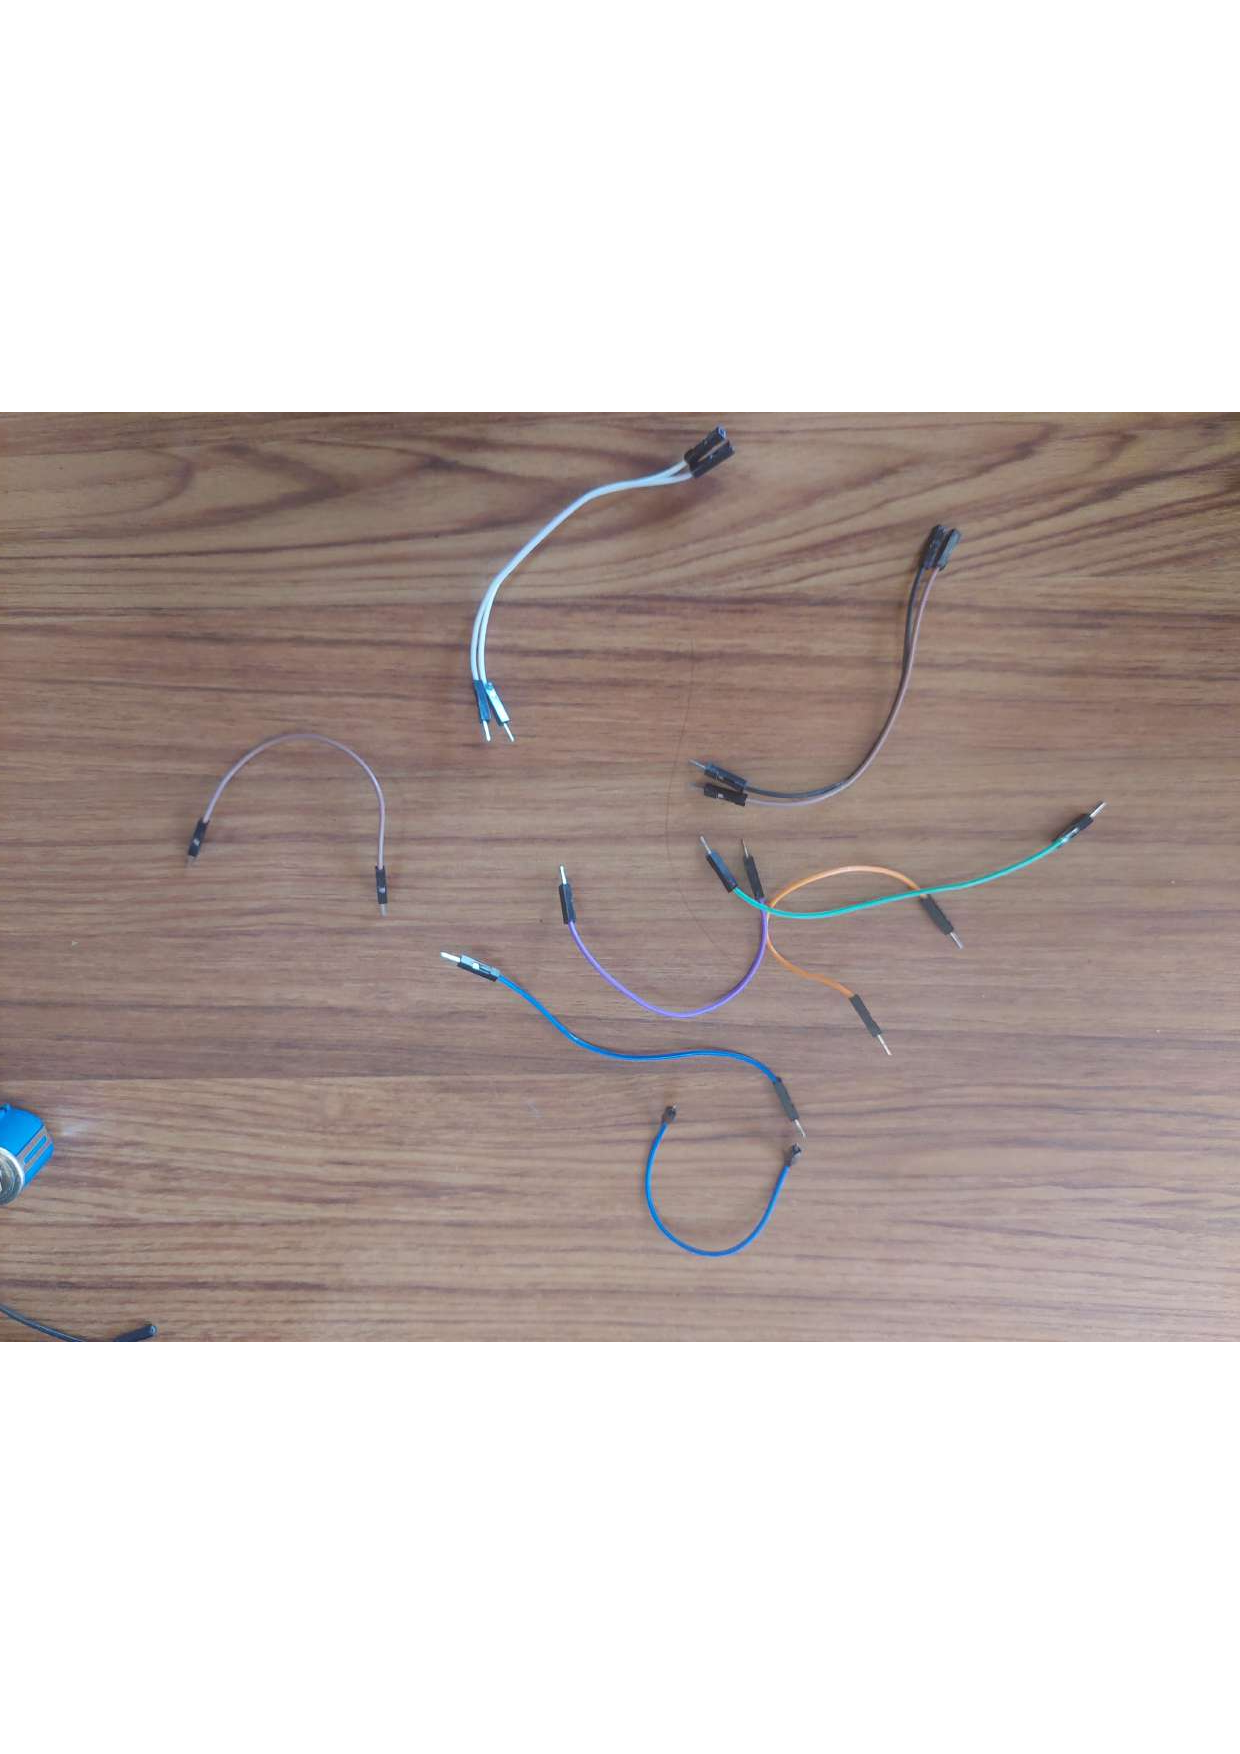
\includegraphics[scale=0.25]{8/Img/Img/Cables dupont.pdf}
    \caption{Cables dupont}
    \label{Cables}
\end{figure}
    \item Resistencias: Las resistencias son esenciales para facilitar el flujo adecuado de corriente. La resistencia sirve como un indicador que cuantifica qué tan rápido fluirá la corriente en un circuito utilizando ohmios como unidad.
    \item Protoboard: Es una herramienta simple que se usa en proyectos de robótica que permite conectar fácilmente componentes electrónicos entre sí, sin necesidad de realizar una soldadura.
    \item Arduino: Utilizado como un microcontrolador, cuando tiene un programa descargado desde un ordenador y funciona de forma independiente de éste, y controla y alimenta determinados dispositivos y toma decisiones de acuerdo al programa descargado e interactúa con el mundo físico gracias a sensores y actuadores.
    \item Potenciametro: Componente electrónico similar a los resistores pero cuyo valor de resistencia en vez de ser fijo es variable, permitiendo controlar la intensidad de corriente a lo largo de un circuito conectándolo en paralelo ó la caida de tensión al conectarlo en serie.
    \item Display: Dispositivo de ciertos aparatos electrónicos que permite mostrar información al usuario de manera visual o táctil.
\end{enumerate}

\subsection{Ensamble}
\begin{enumerate}
    \item Se instalara el arduino en el protoboard ensamblandolo en la linea con la letra b, insertandolo de izquiera a derecha 
    \item Tomaremos un cable dupont y lo colocaremos en el pin numero 7 del arduino, el otro extremo se colocara en la fila con la letra g dejando 2 espacios de donde termina el arduino
    \item Tomaremos otro cable dupont y lo colocaremos en el pin numero 6 del arduino, el otro extremo se colocara al lado derecho del cable dupont colocado anteriormente, dejando un espacio a su derecha
    \item Tomaremos otro cable dupont el cual se colocara en el pin con descripcion 3v3 del arduino, el otro extremo se instalara del lado positivo del protoboard en el segundo espacio de derecha a izquierda 
    \item Tomaremos otro cable dupont y lo colocaremos en el pin con descripcion G del arduino, el otro extremo se colocara en el primer espacio de izquierda a derecha del lado negativo 
\subsection{conexiones de display}   
    \item Tomaremos otro cable dupont el cual se colocara debajo del cable protoboard del segundo paso, el otro extremo se instalara en la parte trasera del display en el pin con descripcion SCL
    \item Tomaremos un nuevo cable dupont el cual se colocara debajo del cable dupont del tercer paso, el otro extremo se instalara en la parte trasera del display en el pin con descripcion SDA
    \item Tomaremos otro cable dupont el cual se colocara en el sexto espacio de derecha a izquiera del lado negativo del protoboard, el otro extremo se instalara en la parte trasera del display en el pin con descripcion GND
    \item Tomaremos otro cable dupont el cual se colocara arriba del cable dupont del paso anterior, el otro extremo se instalara en la parte trasera del display en el pin con descripcion VCC
\subsection{conexiones de potenciometro}
    \item Tomaremos un cable dupont el cual se colocara del lado positivo en el primer espacio de derecha a izquierda, el otro extremo se conectara con un nuevo cable dupont, el extremo sobrante se soldara al potenciometro 
    \item Tomaremos otro cable dupont el cual se colocara debajo del cable dupont del paso anterior, el cual terminara del lado negativo, el extremo de este se conectara de igual manera a un nuevo cable dupont y el extremo sobramte tambien se soldara al potenciometro
    \item Se conectara un ultimo cable dupont en el protoboard el cual ira en el pin 0 del arduino, posteriormente se soldara al potenciometro
\subsection{Resistencias}
    \item La primera resistencia se conectara debajo del cable dupont del paso numero 6 y el otro extremo se colocara en el lado positivo a 7 espacio a la izquierda del cable dupont del paso numero 9
    \item La segunda resistencia se colocara debajo del cable dupont del paso numero 7 dejando un espacio de separacion, el otro extremo se colocara del lado positivo del protoboard a la derecha de la resistencia del paso pasado dejando un espacio de separacion
\subsection{conexiones de multicontacto}
    \item Se conectara un cable con 2 entradas tipo usb, un extremo se conectara en el arduino y el otro extremo se conectara al multicontacto
    \item Por ultimo se enchufara el multicontacto a una conexion de electricidad y se encendera 
\end{enumerate}
\include{5/leonardoBonilla}

\end{document}
